This is a test case on a unit cube (uniaxial strain) with the following manufactured solutions:
\begin{align}
\label{eq:MMS_Solutions}
  \begin{aligned}
    &u(X,t) &&= X^2t^3\, ,\\
    &u_\rf(X,t) &&= \frac{1}{2}X^2t^3\, ,\\
    &p_\rf(X,t) &&= (H - X)t^2
  \end{aligned}
\end{align}
The finite element method is used to solve the following strong-form governing equations:
\begin{align}
\label{eq:Variational_Strong-Forms-MMS}
    \begin{aligned}
        &\DDiv{\bP} + \rho_0\bg - \left(\rho_0^\rs\ba + \rho_0^\rf\ba_\rf\right) = \bzero\, ,\\
        &\bu(\bX, t) = \bg^u(\bX,t)\, \forall \, \bX \in \Gamma_0^u\, ,\\
        &\bP(\bX, t) \cdot \bN(\bX) = \bt^\sigma(\bX,t) \, \forall \, \bX \in \Gamma_0^t\, ,\\
        &\rho_0^\rf\ba_\rf + Jn^\rf\GGrad(p_\rf)\cdot\bF^{-1} + J\frac{\left(n^\rf\right)^2}{\hat{k}}(\bv_\rf - \bv) - \rho_0^\rf\bg = \bzero\, ,\\
        &\bu_\rf(\bX,t) = \bg^{u_\rf}(\bX,t) \, \forall \, \bX \in \Gamma_0^{u_\rf}\, ,\\
        &\frac{J^2 n^\rf}{K^\eta_\rf}\dt{p_\rf} + \dt{J} + \frac{J^2}{K^\eta_\rf}\GGrad(p_\rf)\cdot\bF^{-1}\cdot(n^\rf\tilde{\bv}_\rf) + J\GGrad{(n^\rf\tilde{\bv}_\rf)}\cddot\bF^{-T} = 0\, ,\\
        &p_\rf(\bX,t) = g^{p_\rf}(\bX,t)\, \forall \, \bX \in \Gamma_0^{p_\rf}\, ,\\
        &-[J\bF^{-1}\cdot(n^\rf\tilde{\bv}_\rf)]\cdot\bN(\bX) = Q_\rf(\bX,t)\, \forall \, \bX \in \Gamma_0^{Q_\rf}\, ,
    \end{aligned}
\end{align}
which, under the assumption of 1-D uniaxial strain, uni-directional pore fluid flow, reduce to
\begin{align}
\label{eq:Variational_Strong-Forms-1D-MMS}
    \begin{aligned}
        &\frac{\partial P_{11}}{\partial X} - \rho_0g - \left(\rho_0^\rs a + \rho_0^\rf a_\rf\right) = 0\, ,\\
        &u(X, t) = g^u(X,t)\, \forall \, X \in \Gamma_0^u\, ,\\
        &P_{11}(X, t) = t^\sigma(X,t) \, \forall \, X \in \Gamma_0^t\, ,\\
        &\rho_0^\rf a_\rf + n^\rf\frac{\partial p_\rf}{\partial X} + J\frac{\left(n^\rf\right)^2}{\hat{k}}(v_\rf - v) + \rho_0^\rf g = 0\, ,\\
        &u_\rf(X,t) = g^{u_\rf}(X,t) \, \forall \, X \in \Gamma_0^{u_\rf}\, ,\\
        &\frac{J^2 n^\rf}{K^\eta_\rf}\dt{p_\rf} + \dt{J} + \frac{J}{K^\eta_\rf}\frac{\partial p_\rf}{\partial X}(n^\rf\tilde{v}_\rf) + \frac{\partial(n^\rf\tilde{v}_\rf)}{\partial X} = 0\, ,\\
        &p_\rf(X,t) = g^{p_\rf}(X,t)\, \forall \, X \in \Gamma_0^{p_\rf}\, ,\\
        &-[(n^\rf\tilde{v}_\rf)] = Q_\rf(X,t)\, \forall \, X \in \Gamma_0^{Q_\rf}\, .
    \end{aligned}
\end{align}
For elastodynamics applications, only Eqs.~\eqref{eq:MMS_Solutions}$_1$,\eqref{eq:Variational_Strong-Forms-1D-MMS}$_{1,2,3}$ are considered.\\

The constitutive model for the $\OneField$ formulation (single-phase model) is classical neo-Hookean, such that
\begin{align}
    \begin{aligned}
        &P_{iI} &&\defeq \mu F_{iI} + (\lambda\ln(J) - \mu)F_{Ii}^{-1}\, ,\\
        &\frac{\partial P_{iI}}{\partial X_I} &&= \mu\frac{\partial^2 u_i}{\partial X_I^2} + \lambda F_{Ii}^{-1}\Big(F_{Ii}^{-1}\frac{\partial^2 u_i}{\partial X_I^2}\Big) - (\lambda\ln(J) - \mu)F_{Ii}^{-2}\frac{\partial^2 u_i}{\partial X_I^2}\, .
    \end{aligned}
\end{align}
For the $\ThreeField$ formulation (multiphase model), this is extended to the finite-strain model for incompressible solid developed by \citet{Ehlers-Eipper1999}, such that
\begin{align}
    \begin{aligned}
		&P_{iI(E)}^\rs \defeq \mu F_{iI} + \Big(\lambda(1 - n_0^\rs)^2\Big[\dfrac{J}{1 - n_{0}^\rs} - \dfrac{J}{J - n_{0}^\rs}\Big] - \mu\Big)F_{iI}^{-1} - Jp_\rf F_{Ii}^{-1}\, ,\\
        &\frac{\partial P_{iI}}{\partial X_I} = \mu\frac{\partial^2 u_i}{\partial X_I^2}(1 + F_{Ii}^{-2}) + \lambda(1 - n_0^\rs)^2\frac{\partial^2 u_i}{\partial X_I^2}\Big[F_{Ii}^{-1}\Big(\frac{J F_{Kk}^{-1}}{1 - n_0^\rs} + \frac{Jn_0^\rs F_{Kk}^{-1}}{(J - n_0^\rs)^2}\Big)\\
        &\phantom{\frac{\partial P_{iI}}{\partial X_I} =} - F_{Ii}^{-2}\Big(\frac{J}{1 - n_0^\rs} - \frac{J}{J - n_0^\rs}\Big)\Big] - \frac{\partial p_\rf}{\partial X}\, .
    \end{aligned}
\end{align}
Additionally, the hyperbolic hydraulic conductivity model developed by \citet{Markert2005} is preferred over a standard Kozeny-Carman model since the former is well suited for finite strains (which one encounters in MMS):
\begin{align}
    \hat{k} \defeq \frac{\varkappa}{\mu_\rf}\Big(\frac{J - n_0^\rs}{1 - n_0^\rs}\Big)^\kappa\, .
\end{align}
Per the analytical solutions given by Eq.~\eqref{eq:MMS_Solutions}, the following boundary conditions are prescribed:
{\footnotesize
\begin{align}
\label{eq:MMS-BCs-1D}
    \begin{aligned}
        &g^u(X=0,t) &&= 0\, ,\\
        &t^\sigma(X = H,t) &&= \mu\Big(1 + 2Ht^3 - \frac{1}{1 + 2Ht^3}\Big) + \lambda(1 - n_0^\rs)^2\Big(\frac{1}{1 - n_0^\rs} - \frac{1}{2Ht^3 - n_0^\rs}\Big) \, ,\\
        &g^{u_\rf}(X = 0,t) &&= 0 ,\\
        &g^{p_\rf}(X = 0,t) &&= Ht^2 ,\\
        &Q_\rf(X = H,t) &&=  -\frac{\varkappa}{\mu_\rf}\Big(\frac{1 + 2Ht^3 - n_0^\rs}{1 - n_0^\rs}\Big)^\kappa\Big(\frac{\rhofr_0}{K_\rf^\eta}Ht^2[6X^2t + g] + \frac{t^2}{1 + 2Ht^3}\Big).
    \end{aligned}
\end{align}}%

Below are two temporal convergence plots, which demonstrate convergence of the implicit solvers.

\begin{figure}[htb!]
\centering
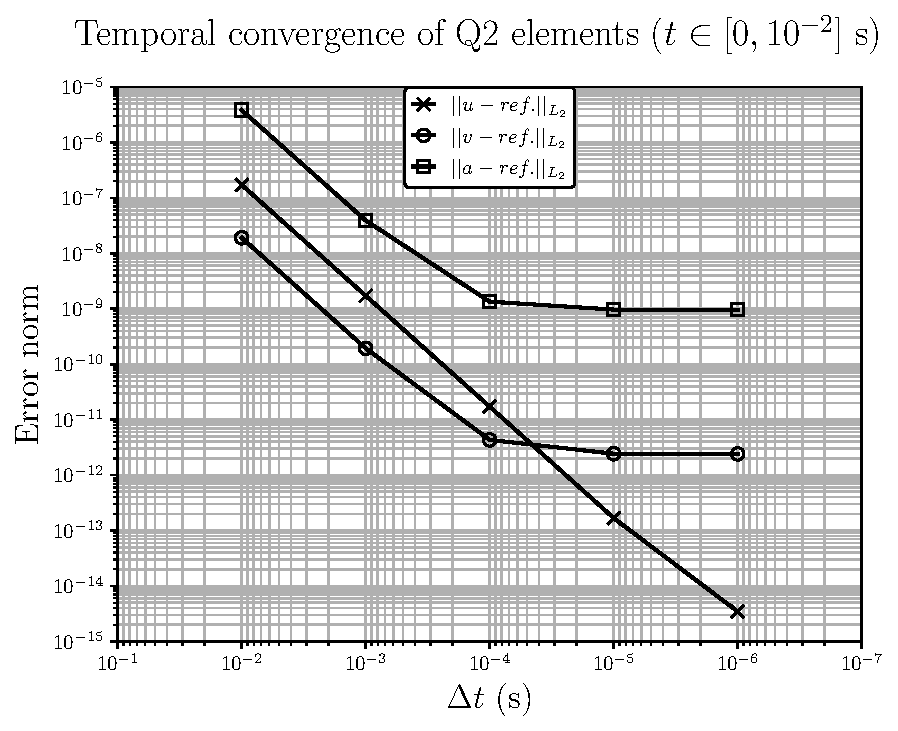
\includegraphics[width=0.7\textwidth]{./Cases/MMS/figures/u_t_L2.pdf}
\end{figure}
\begin{figure}[htb!]
\centering
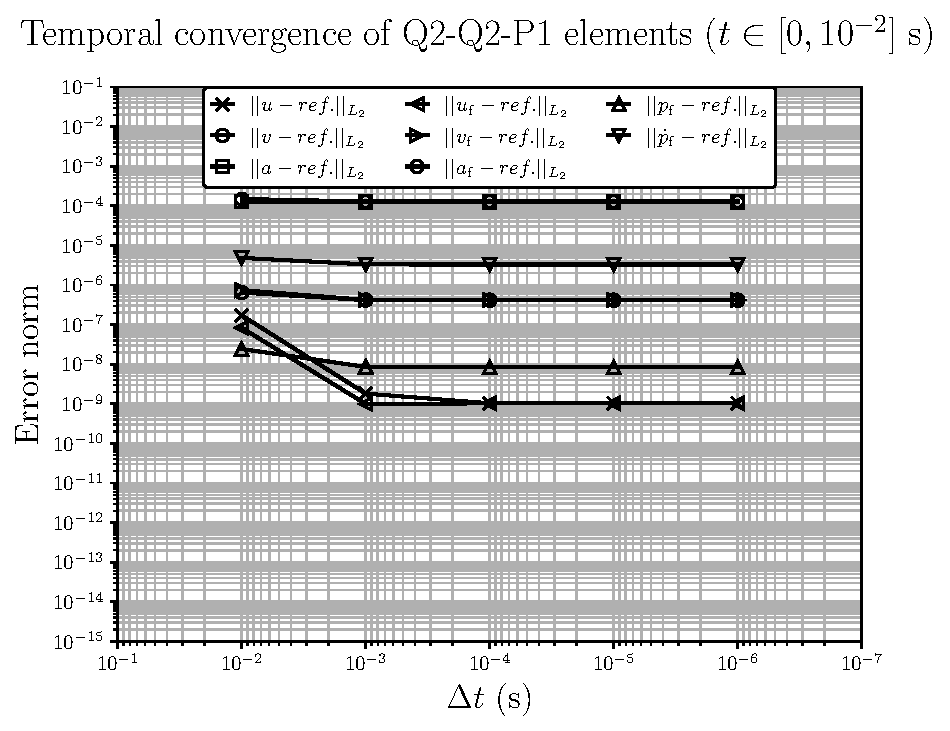
\includegraphics[width=0.7\textwidth]{./Cases/MMS/figures/uufpf_t_L2.pdf}
\end{figure}
